\subsection{Struktur des Modells}

Die Struktur des Modells für Erklärungen orientiert sich an den Forschungsfragen und Anforderungen an das Modell, Ergebnissen aus der Literaturrecherche sowie dem bestehenden Konzept der Qualitätsmodelle \cite{schneider2012abenteuer} (Siehe \autoref{sec:basics_quality_models}).

In der Literatur wurden einige Aspekte des Modells nicht nur verschieden genannt, sondern auch zum Teil in Oberkategorien gegliedert oder auf verschiedenen Abstraktionsebenen betrachtet. Hieraus ergibt sich eine Hierarchische Anordung des Modells. Verschiedene Abstraktionsebenen enthalten auch die von \citeauthor{schneider2012abenteuer} vorgestellten Qualitätsmodelle \cite{schneider2012abenteuer}. Dabei werden abstrakte Ziele (\textit{Objectives}) immer weiter konkretisiert, bis sie schlussendlich mit konkreten Metriken messbar sind. Das zugrunde liegende Modell (\glqq Goal-Driven and Property-Based Definition Approach for Product Metrics\grqq{} \cite{briand1995goal}) von \citeauthor{briand1995goal} definiert außerdem unter anderem die nötigen Abhängigkeiten der \textit{Objectives} von äußeren Faktoren, die im hier vorgestellten Modell für Erklärungen dem bereits erwähnten \textit{Context} entsprechen.

Die Betrachtung von \textit{Context} und \textit{Objectives} erfolgt in der Literaur über Erklärungen zum Teil in verschiedener Reihenfolge. \citeauthor{rosenfeld_explainability_2019} schreiben, dass die erste Frage, welche geklärt werden sollte, die Frage \glqq Warum benötigt das System eine Erklärung?\grqq{} ist \cite[vgl. S. 699][]{rosenfeld_explainability_2019}\cite{nunes_systematic_2017}. Im Gegensatz dazu schreiben \citeauthor{cirqueira_scenario-based_2020}, dass zuerst äußere Umstände, wie der Endnutzer des Systems geklärt sein sollte (\glqq Stakeholder Setting\grqq{} \cite{cirqueira_scenario-based_2020}), um darauf aufbauend die Ziele festzulegen. Hieraus wird geschlussfolgert, dass die Festlegung der Ziele mit ihren Abhängigkeiten wie auch von \cite{schneider2012abenteuer} geschildert eine iterative, stark zusammenhängende Aufgabe ist. Daher werden die Punkte \textit{Context} und \textit{Objectives} aus \autoref{tab:model_explaination_aspects} unter \textit{External Dependencies} zusammengefasst. Dies verdeutlicht, dass die \textit{Objectives} für das Integrieren von Erklärungen stark mit anderen äußeren Einflüssen (\textit{Context}) zusammenhängen (\autoref{sec:model_external_dependencies}).

Auch werden \textit{Demand}, \textit{Content} und \textit{Presentation} vereint dargestellt, da sich diese drei Kategorien direkt auf die Eigenschaften von Erklärungen beziehen (\textit{Characteristics}). Damit wird der Zusammenhang zwischen den verschiedenen Merkmalen einer Erklärung verdeutlicht \cite{nunes_systematic_2017}.

Zusätzlich zur Zielevaluation der Qualitätsmodell betrachtet das Modell die unmittelbare Evaluation von Erklärungen. Diese müssen einzeln betrachtet werden, da für diese die Metriken zum Teil erst nach der Entwicklung der Erklärungen festgelegt werden können.

\smallbreak

Schlussendlich ist die Übersicht in die drei Oberkategorien \textit{External Dependencies}, \textit{Characteristics} und \textit{Evaluation} gegliedert. Eine Übersicht ist in \autoref{fig:model_overview} zu sehen. Die Gesamtübersicht des Modells für Erklärungen bietet \autoref{fig:model_overview_complete}. Diese enthält darüber hinaus die in den folgenden Abschnitten beschriebenen Ausprägungen der einzelnen Kategorien aus der Literatur. Die Gesamtübersicht ist grafisch an der Taxonomie für Erklärungen von \citeauthor{nunes_systematic_2017} angelehnt und enthält auch einige Aspekte daraus \cite{nunes_systematic_2017}. Die erwähnte Taxonomie ist allerdings nur auf den Einsatz von Erklärungen in Empfehlungssystemen bezogen und beschränkt sich daher u.~a. auf bestimmte Darstellungstypen. Sie kann folglich nicht ohne Weiteres in andere Kontexte übertragen werden. Darüber hinaus fehlt der Aspekt der Evaluation. Dieser wird allerdings nicht nur von \citeauthor{nunes_systematic_2017} selbst, sondern auch von weiteren Autoren für wichtig erachtet \cite{cirqueira_scenario-based_2020, martin_evaluating_2021}.

\begin{figure}[htb!]
    \begin{center}
        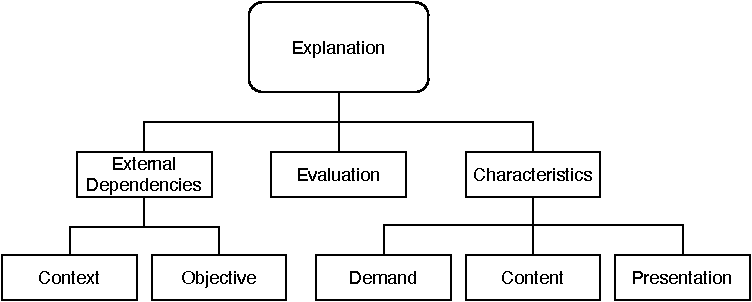
\includegraphics[width=0.9\linewidth]{contents/05_model_description/res/model-overview.pdf}
    \end{center}
    \caption{Oberkategorien der Aspekte von Erklärungen}
    \label{fig:model_overview}
\end{figure}